Here we derive an expression for the Bernoulli parameter, 
\be
\mathcal{B} \equiv \ke
+\gammaf \frac{p}{\rho}+\Phi,
\ee
assuming a stellar density profile $\rhostar\sim r^{-1-\Gamma}=r^{-\delta}$ characteristic of that inside the break radius $\rb$.

Basic manipulation of the equations of hydrodynamics (eqs.~[\ref{eq:drhodt}]-[\ref{eq:dsdt}]) results in the following relationship between the Bernoulli parameter and the net heating rate $\propto q \vw^{2}$,
\begin{align}
\frac{1}{r^2} \frac{d}{dr} \left(r^2 \rho v \mathcal{B} \right) = q \kew + q \Phi = \frac{3}{1+\delta}\frac{G
  \Mbh}{r}+\sigma_0^2+v_w^2 + q \Phi,
\label{eq:enCons}
\end{align}
where the first and second terms on the right hand side correspond, respectively, to the black hole and stellar contributions to the velocity dispersion.

Integrating both sides of equation~\eqref{eq:enCons} from the stagnation radius $r = \rs$ outwards,
\begin{align}
  r^2 \rho v \left(\ke+\Phi+\gammaf \frac{p}{\rho} \right)= \int_{\rs}^{r}
    r^2 \left(q \kew + q\Phi\right) dr
    \label{eq:enConsInt}
\end{align}
From mass continuity (eq.~[\ref{eq:drhodt}]) the mass flux can be written
\be
 f\equiv r^2 \rho v = q_o \rs^3 \left[\frac{x^{3-\delta}-1}{3-\delta}\right],
 \label{eq:massFlux}
\ee
where $x \equiv r/\rs$ and we have used the fact that the mass source term $q = q_o x^{-\delta}$ is proportional to the stellar density.  Likewise, the gravitational potential $\Phi$ is given by
\begin{align}
\Phi \simeq -\frac{G \Menc}{r} -4 \pi G \int_{r}^{\rb} \rhostar(r') r' dr',
\label{eq:Phi}
\end{align}
where by truncating the integral at $r = \rb$ we are neglecting the contribution to the potential of the stars outside of the break radius.

Combining equations~\eqref{eq:enConsInt} and \eqref{eq:massFlux} with the result of equation \eqref{eq:Phi}, we obtain 
\begin{align}
  &\mathcal{B} = -U_o\left[\frac{\rs/\rb}{2-\delta}-\frac{x^{5-2\delta}-1}{x^{3-\delta}-1}\frac{3-\delta}{(5-2\delta)(2-\delta)}\right]\nonumber\\
  &+\frac{v_w^2}{2}+\frac{\sigma_0^2}{2}- \frac{G \Mbh}{r_s}
  \frac{1-2\delta}{2(\delta+1)} \frac{3-\delta}{2-\delta}\frac{x^{2-\delta}-1}{x^{3-\delta}-1}
  \nonumber\\
  &-\frac{G M_\star}{r_s}
  \frac{x^{5-2\delta}-1}{x^{3-\delta}-1}\frac{3-\delta}{5-2\delta},
\end{align}
where $U_o=4 \pi G \rhostar(\rs) \rs^2$.  We may rewrite this as 

\begin{multline}
  \mathcal{B} =\frac{G \Mbh}{\rs} 
\biggl[
  \frac{3}{2} \zeta^2 w^{\frac{1}{3 -\delta}}
  -\frac{(1-2\delta)(3-\delta)}{2(\delta+1)(2-\delta)}  \frac{x^{2  -\delta}-1}{x^{3-\delta}-1}\\
  -\frac{\rb}{\rsoi} w^{\frac{\delta-1}{3-\delta}} \frac{3 -\delta}{2 -\delta} 
  -w \frac{(2-\delta)(3-\delta)-(3-\delta)^{2}}{(5-2\delta)(2-\delta)} \frac{x^{5-2\delta}-1}{x^{3-\delta}-1}
\biggr],
\label{eq:enthAnal}
\end{multline}
where $\zeta \equiv \sqrt{v_w^2+\sigma_0^2}/\sigma_0$ and $w\equiv (\rs/\rsoi)^{3\delta}$, and
$\delta$ is the power law slope of the stellar density profile inside
of the break radius, $\rb$.

When the rate of external heating is high, we have $\mathcal{B} > 0$ at all radii, requiring an outflow.  As heating ($\zeta$) is decreased, there exists a critical value of $\zeta = \zeta_{c}$ below which $\mathcal{B}$ first becomes negative.  If $\zeta<\zeta_c$, then there is a minimum value of $\rs/\rsoi$, $(\rs/\rsoi)_{\rm min}$, above which we have $\mathcal{B} > 0$ at the break radius, allowing an outflow with positive kinetic energy at infinity.  The value of $\zeta_c$ is an increasing function of $r_{b}/r_{\rm soi}$ since a greater heating rate is required to unbind gas from a deeper stellar potential (Fig.~\ref{fig:zetaCrit}).  Specifically, we find $\zeta_c\sim (\rb/\rsoi)^{0.5(1-\Gamma)}$ for $\rb\gsim\rsoi$ (see the top panel of
Fig.~\ref{fig:zetaCrit}). Likewise $(r_{\rm s}/r_{b})_{\rm min}$ is an increasing function of $\zeta/\zeta_{c}$, approaching unity for $\zeta < 0.5\zeta_c$ {\bf BDM: put in the right numbers here}.  For values of $\zeta<\zeta_c$, the stagnation radius rapidly approaches the break radius as shown in the
bottom panel of Fig.~\ref{fig:zetaCrit}.

\begin{figure}
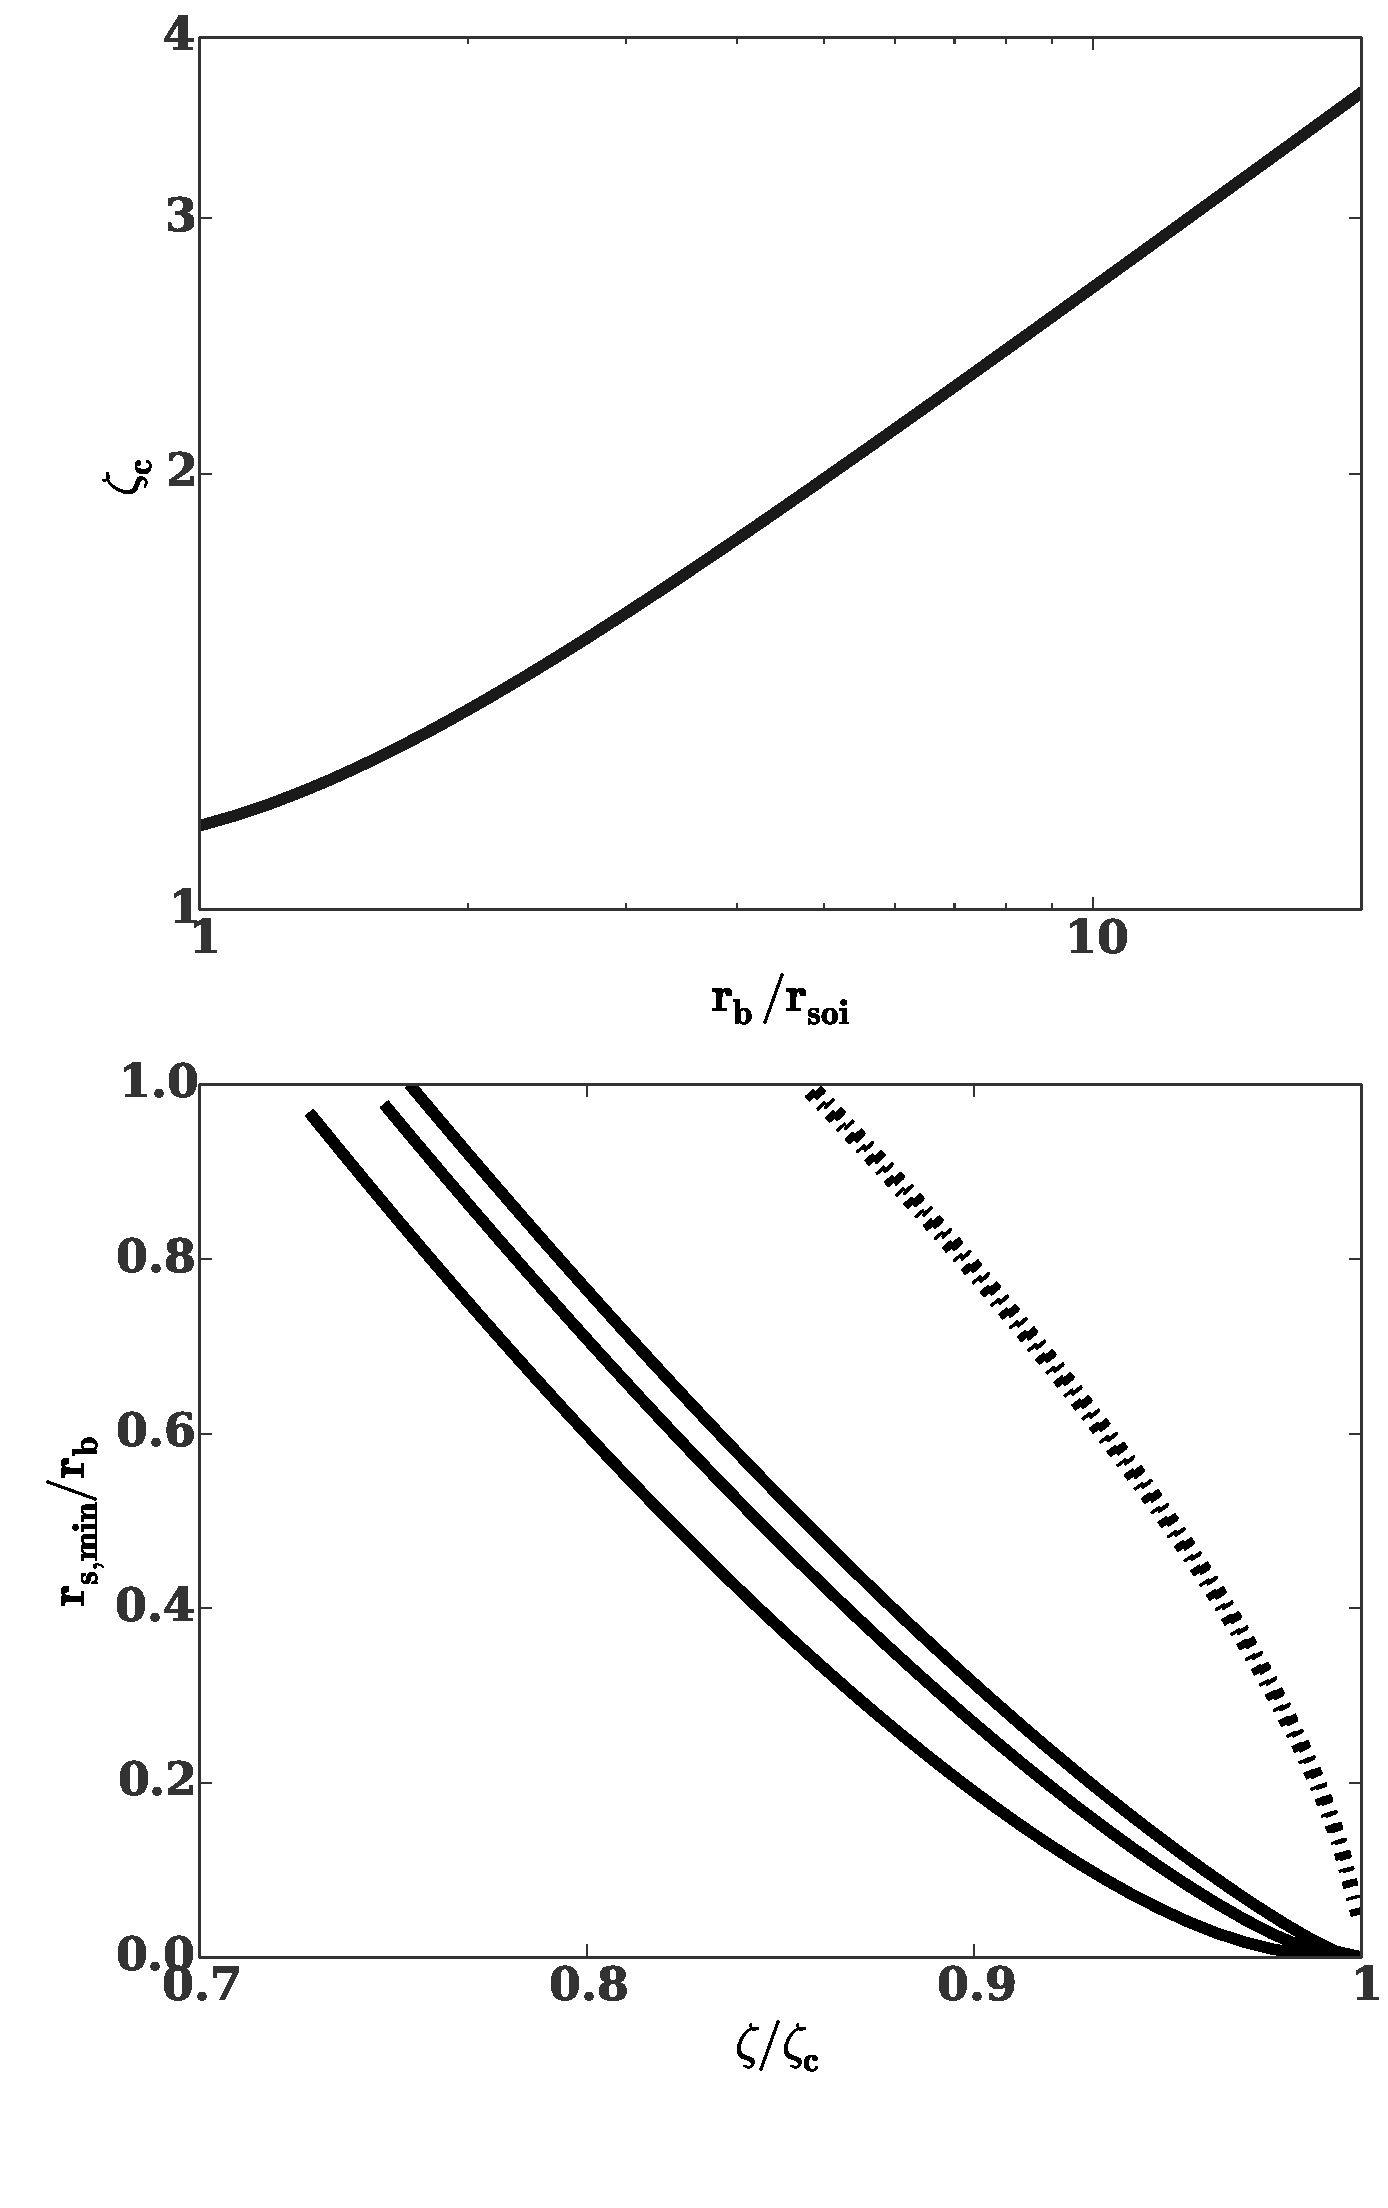
\includegraphics[width=\columnwidth]{zetaCrit.pdf}
\caption{\label{fig:zetaCrit} {\emph Top panel:} Critical
  $\zeta_c=\sqrt{v_w^2+\sigma_0^2}/\sigma_0$. If $\zeta<\zeta_c$ outflows are
  only possible if the ratio of the stagnation radius to the influence
  radius exceeds a minimum value. Plotted as a function of the ratio
  of the break radius to the influence radius ($\rb/\rsoi$) {\emph Bottom
    Panel:} Mininmum value for ratio of the stagnation radius to the
  influence radius, $\rs/\rsoi$ for core galaxies ($\Gamma=0.1$)
  derived by requiring enthalpy of the gas to remain positive out to
  the break radius $\rb$. This is calculated numerically from
  equation~\eqref{eq:enthAnal}. The x-intercept of each curve
  corresponds to the critical $\zeta_c$}
\end{figure}


%%% Local Variables: 
%%% mode: latex
%%% TeX-master: "ms"
%%% End: 
